%
% Licensed to the Apache Software Foundation (ASF) under one
% or more contributor license agreements.  See the NOTICE file
% distributed with this work for additional information
% regarding copyright ownership.  The ASF licenses this file
% to you under the Apache License, Version 2.0 (the
% "License"); you may not use this file except in compliance
% with the License.  You may obtain a copy of the License at
%
%   http://www.apache.org/licenses/LICENSE-2.0
%
% Unless required by applicable law or agreed to in writing,
% software distributed under the License is distributed on an
% "AS IS" BASIS, WITHOUT WARRANTIES OR CONDITIONS OF ANY
% KIND, either express or implied.  See the License for the
% specific language governing permissions and limitations
% under the License.
%
\documentclass[convert={density=300,size=500x500,outext=.png}]{standalone}
\usepackage{tikz}
\usepackage{pgf}
\usetikzlibrary{arrows,positioning}
\usepackage{graphicx}
\tikzset{
    procs/.style={
           rectangle,
           rounded corners,
           draw=black, thick,
           text width=13em,
           minimum height=.5em,
           text centered},
    % Define arrow style
    msgs/.style={
           ->,
           thick,
           shorten <=2pt,
           shorten >=2pt,}
}
\begin{document}
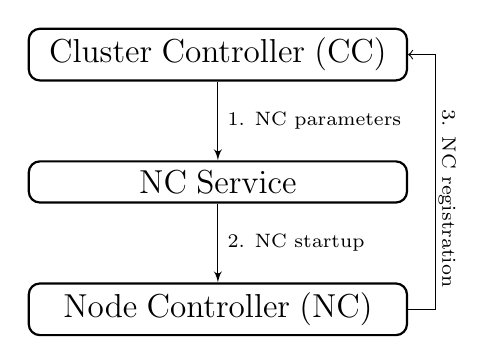
\begin{tikzpicture}[node distance=1cm, auto,]
	\node[procs] (nc) {\large Node Controller (NC)};
	\node[procs,above=of nc] (ncservice) {\large NC Service};
	\node[procs, above= of ncservice] (cc) {\large Cluster Controller (CC)};

	\path [draw, -latex'] (ncservice) -- node {\scriptsize 2. NC startup}(nc);
	\path [draw, -latex'] (cc) --  node {\scriptsize 1. NC parameters }(ncservice);
	\draw [->] (nc.east) -- ++(1em,0) node[near end, rotate=-90,xshift=-4em] {\scriptsize 3. NC registration} |- (cc.east);
\end{tikzpicture} \\*


\end{document}
